\section{Interfejs użytkownika}

W obecnych czasach niezwykle istotnym fragmentem każdego systemu sprzedaży jest
jego interfejs graficzny. Powinien być nie tylko użyteczny ale również, a może
przede wszystkich - atrakcyjny. Takie wymagania spełnia prototyp interfejsu jaki
zostanie zaprezentowany poniżej.

Cały prototyp został wykonany w technologii umożliwającej umieszczenie go w
sieci Internet pod adresem:
\url{http://rowery.hol.es/} \\
Należy jednak pamiętać, iż jest to tylko prototyp interfejsu i nie zawiera
większości funkcjonalności przyszłego systemu, a jedynie prezentuje wygląd jaki
może osiągnąć system. \\

Strona główna sklepu będzie prezentować się jak na rysunku \ref{fig:MainPage}
\begin{figure}[h!]
  \centering
    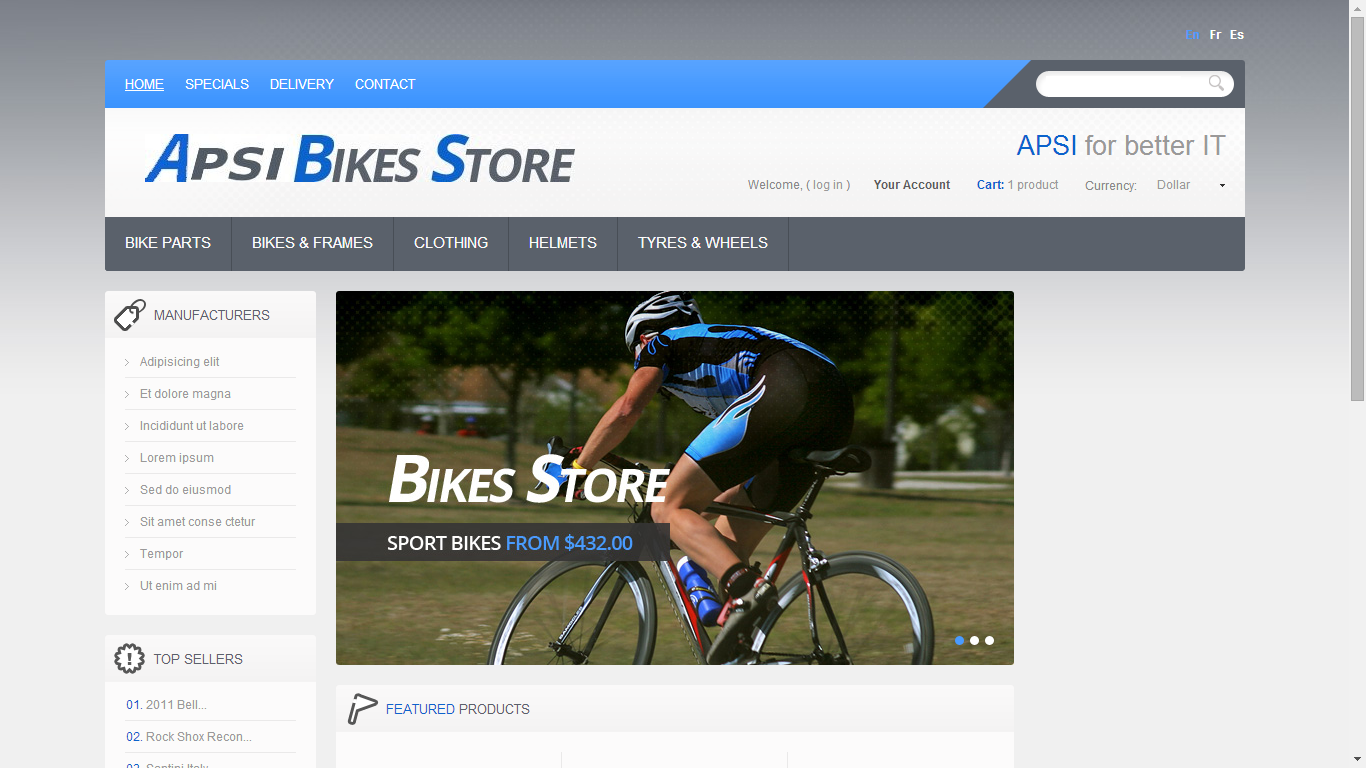
\includegraphics[width=1.0\textwidth]{graphics/ui/MainPageUp.png} 
  \caption{Strona główna sklepu}
  \label{fig:MainPage}
\end{figure}
\begin{figure}[h!]
  \centering
    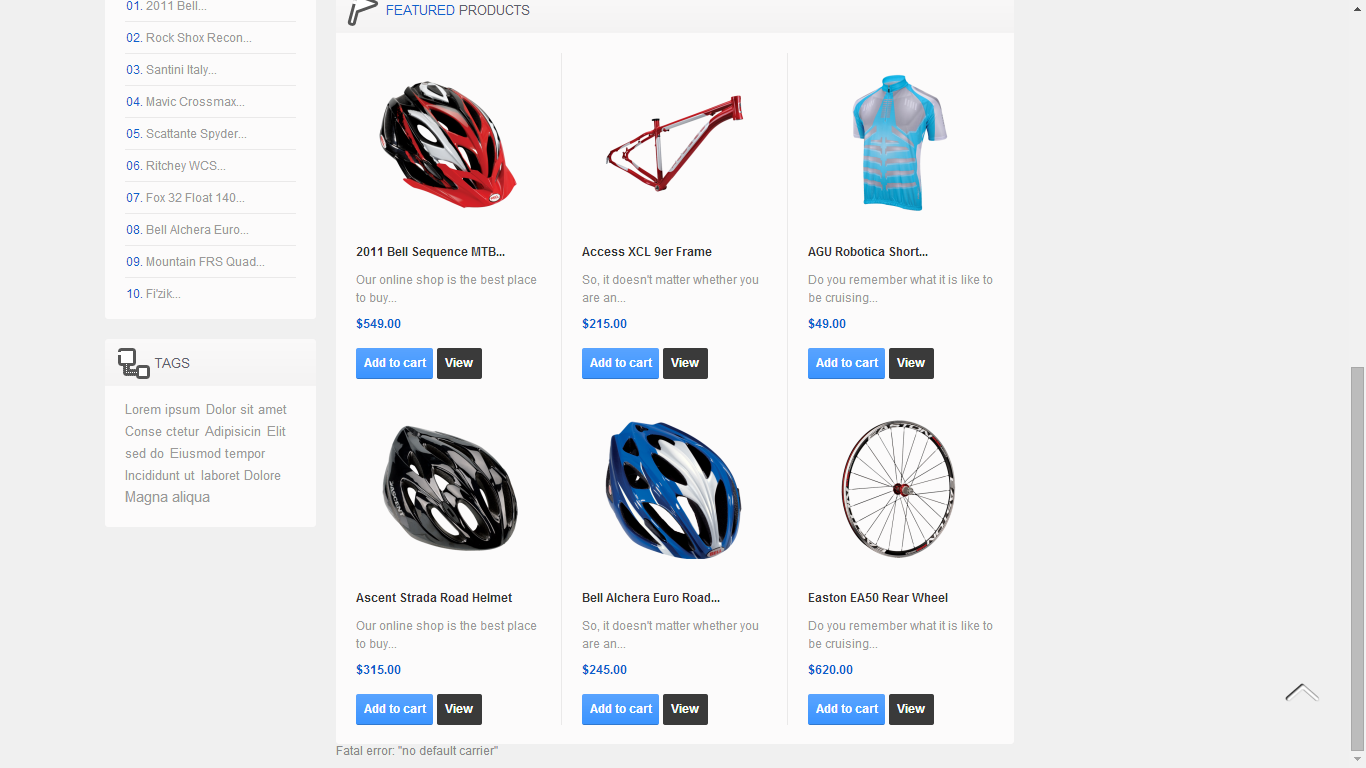
\includegraphics[width=\textwidth]{graphics/ui/MainPageBottom.png}
  \caption{Strona główna zawiera również moduł prezentujący przykładowe
  produkty}
  \label{fig:MainPageBottom}
\end{figure}

Strona główna zawiera również moduł prezentujący przykładowe produkty (Rysunek
\ref{fig:MainPageBottom}). Dzięki temu można bardzo szybko zaintersować klienta.
Sama lista produktów musi zawierać podstawowe informacje oraz zdjęcie każdego z
nich. Obrazy pozwalają na ekspresowe wybranie poszukiwanej rzeczy, natomiast
krótki opis może wystarczyć, by dodać ją do koszyka. Procedura zakupu odbywa się
przez popularny ``Koszyk''. Fragment listy produktów pokazuje Rysunek
\ref{fig:ProductList} \\

\begin{figure}[h!]
  \centering
    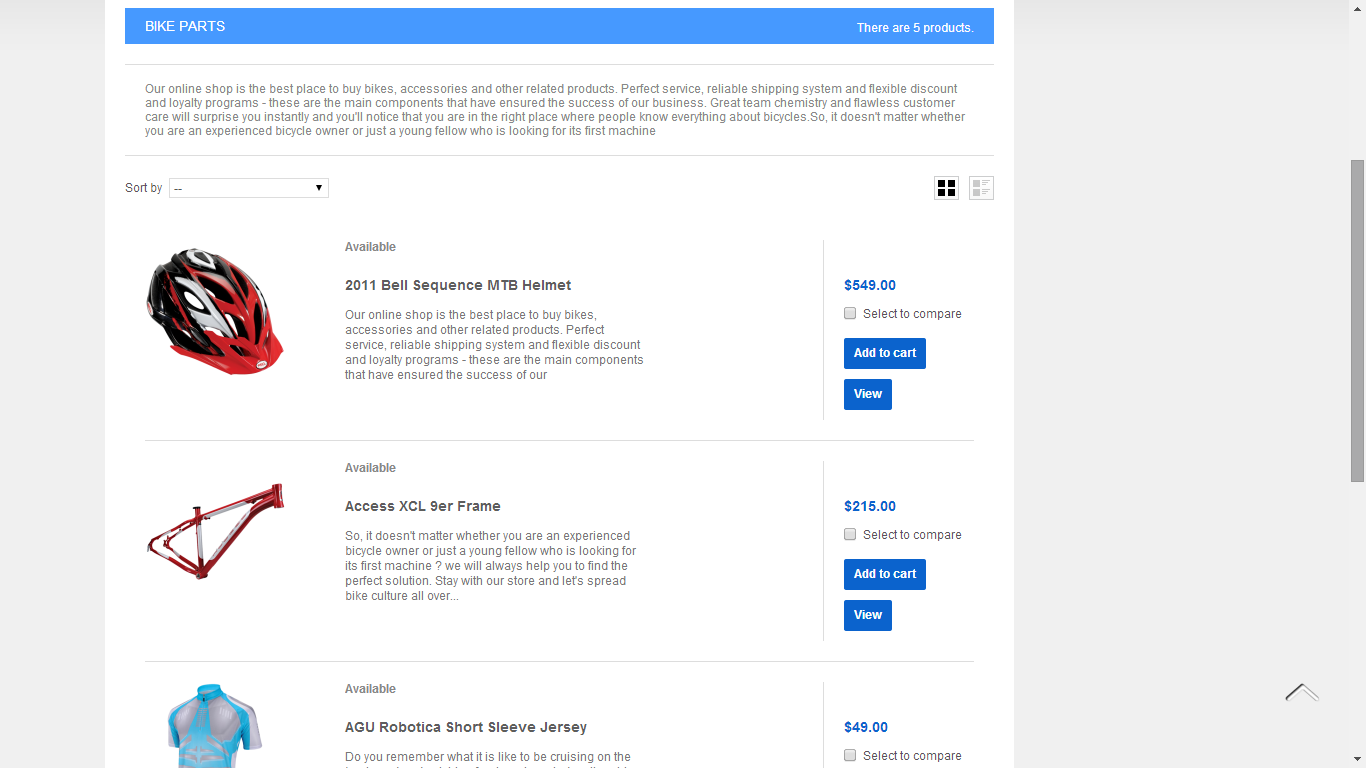
\includegraphics[width=\textwidth]{graphics/ui/Products.png}
  \caption{Fragment listy produktów}
  \label{fig:ProductList}
\end{figure}

W każdym momencie można również sprawdzić szczegóły techniczne danego produktu,
wybierając go z listy produktów, po czym użytkownik widzi nowy ekran z pełnymi
informacjami (Rysunek \ref{fig:ProductPresentation}).

\begin{figure}[h!]
  \centering
    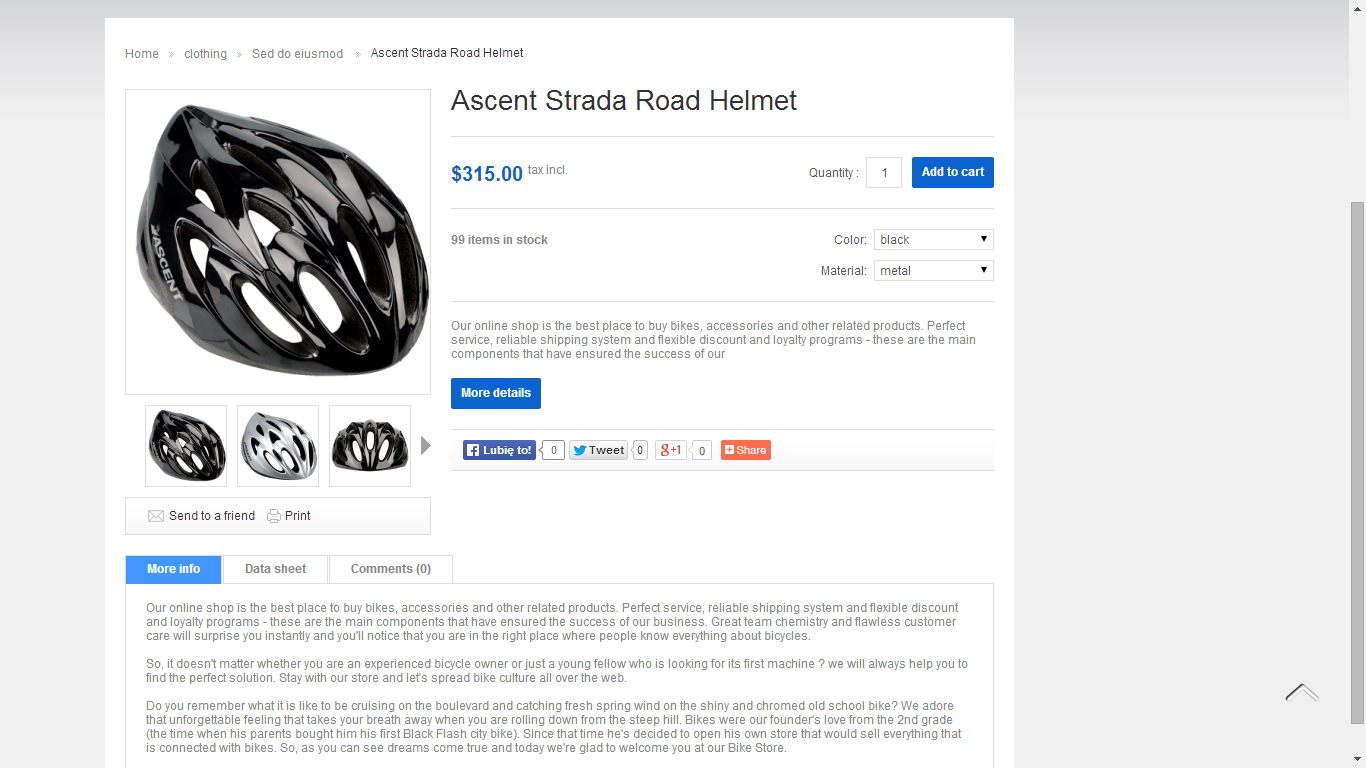
\includegraphics[width=\textwidth]{graphics/ui/ProductPresentation.png}
  \caption{Prezentacja szczegółów dotyczących produktu}
  \label{fig:ProductPresentation}
\end{figure}

\begin{figure}[h!]
  \centering
    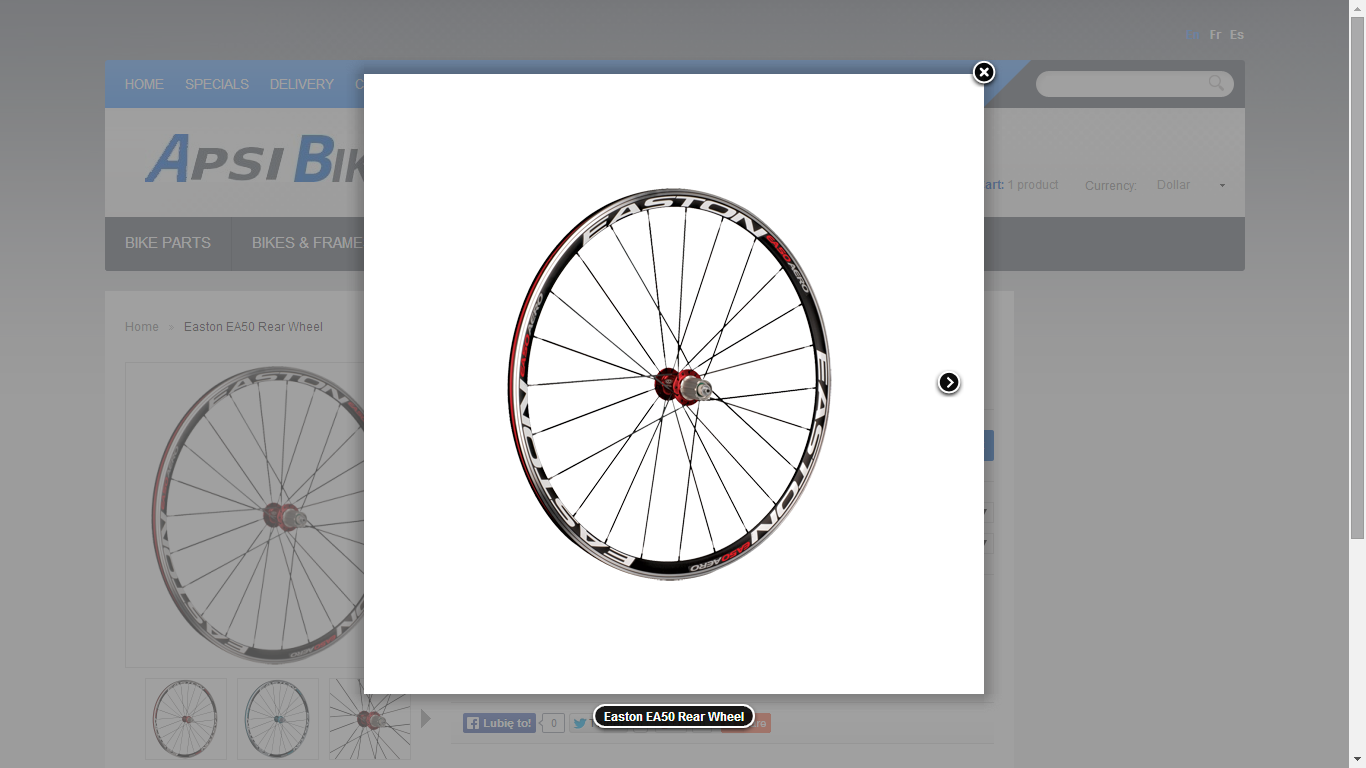
\includegraphics[width=\textwidth]{graphics/ui/ProductImage.png}
  \caption{Powiększony obraz produktu}
\end{figure}

\begin{figure}[h!]
  \centering
    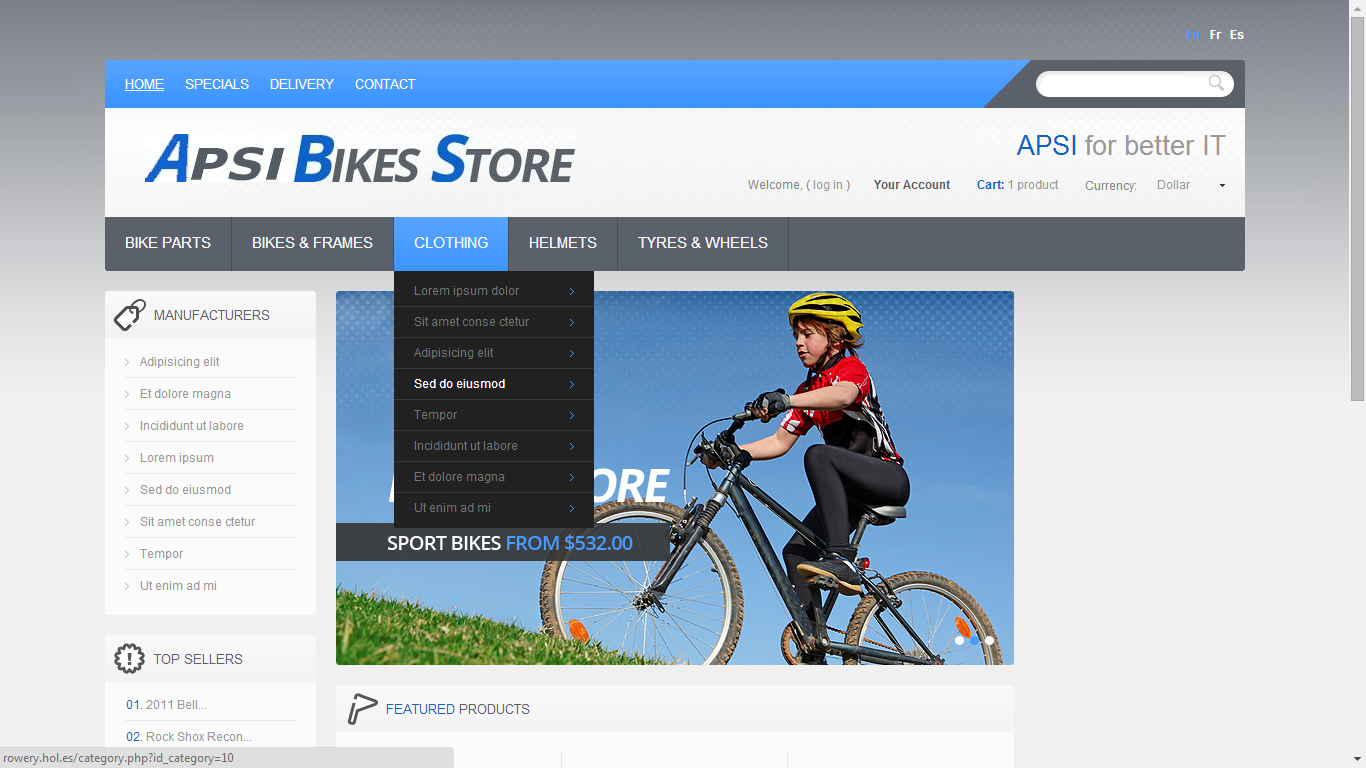
\includegraphics[width=\textwidth]{graphics/ui/MenuPresentation.png}
  \caption{Prezentacja rozwijanego menu}
\end{figure}

\begin{figure}[h!]
  \centering
    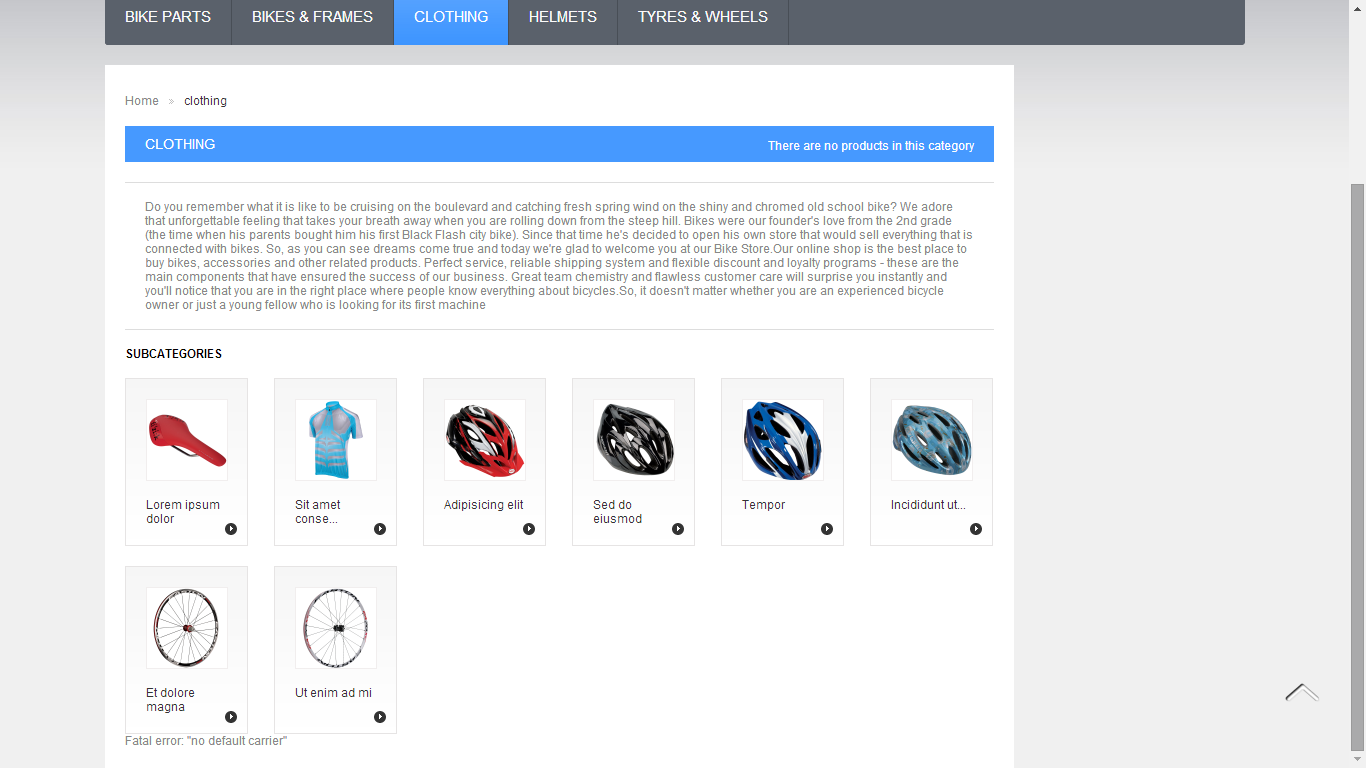
\includegraphics[width=\textwidth]{graphics/ui/Categories.png}
  \caption{Kategorie produktów}
\end{figure}

\begin{figure}[h!]
  \centering
    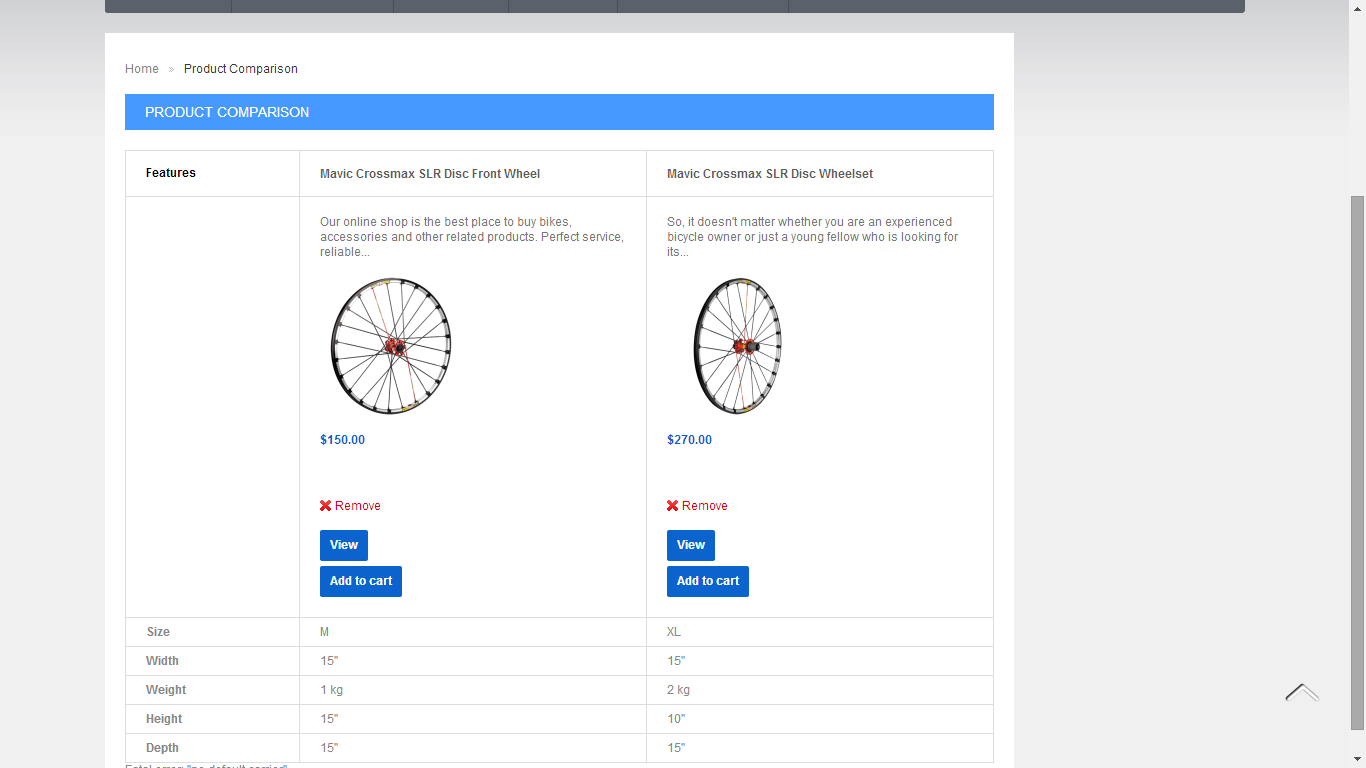
\includegraphics[width=\textwidth]{graphics/ui/ProductComparison.png}
  \caption{Porównywarka produktów}
\end{figure}